\documentclass[border=3pt,tikz]{standalone}
\usepackage{ctex}
\usepackage[utf8]{inputenc}


\usepackage{amsmath} % for \text
\usepackage{etoolbox} % ifthen
\usepackage[outline]{contour} % glow around text
\usetikzlibrary{calc} % for adding up coordinates
\usetikzlibrary{decorations.markings,decorations.pathmorphing}
\usetikzlibrary{angles,quotes} % for pic (angle labels)
\usetikzlibrary{arrows.meta} % for arrow size
\usepackage{xfp} % higher precision (16 digits?)
\contourlength{1.1pt}

\tikzset{>=latex} % for LaTeX arrow head
\colorlet{myred}{red!85!black}
\colorlet{myblue}{blue!80!black}
\colorlet{mygreen}{green!80!black}
\colorlet{mydarkred}{red!55!black}
\colorlet{mylightred}{red!85!black!12}
\colorlet{myfieldred}{mydarkred!5} % for S' background
\colorlet{mydarkblue}{blue!50!black}
\colorlet{mylightblue}{blue!50!black!30}
\colorlet{mylightblue2}{myblue!10}
\colorlet{mypurple}{blue!40!red!80!black}
\colorlet{mydarkgreen}{green!50!black}
\colorlet{mydarkpurple}{blue!40!red!50!black}
\colorlet{myorange}{orange!40!yellow!95!black}
\colorlet{mydarkorange}{orange!40!yellow!85!black}
\colorlet{mybrown}{brown!20!orange!90!black}
\colorlet{mydarkbrown}{brown!20!orange!55!black}
\tikzstyle{world line}=[myblue!40,line width=0.3]
\tikzstyle{world line t}=[mypurple!50!myblue!40,line width=0.3]
\tikzstyle{world line'}=[mydarkred!40,line width=0.3]
\tikzstyle{mysmallarr}=[-{Latex[length=3,width=2]},thin]
\tikzstyle{mydashed}=[dash pattern=on 3 off 3]
\tikzstyle{rod}=[mydarkbrown,draw=mydarkbrown,double=mybrown,double distance=2pt,
                 line width=0.2,line cap=round,shorten >=1pt,shorten <=1pt]
\tikzstyle{vector}=[->,line width=1,line cap=round]
\tikzstyle{vector'}=[vector,shorten >=1.2]
\tikzstyle{particle}=[mygreen,line width=0.9]
\tikzstyle{photon}=[-{Latex[length=5,width=4]},myorange,line width=0.8,decorate,
                    decoration={snake,amplitude=1.0,segment length=5,post length=5}]

\def\tick#1#2{\draw[thick] (#1) ++ (#2:0.06) --++ (#2-180:0.12)}
\def\tickp#1#2{\draw[thick,mydarkred] (#1) ++ (#2:0.06) --++ (#2-180:0.12)}
\def\Nsamples{100} % number samples in plot

\begin{document}

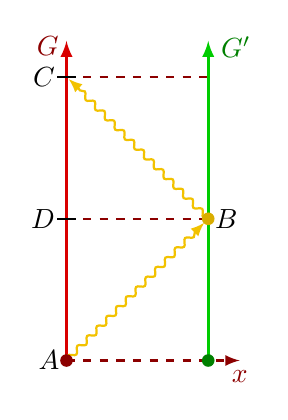
\begin{tikzpicture}[scale=2.0]
  \message{Two observers^^J}
  
  \def\xmin{0.2}
  \def\xmax{2}
  \def\R{2.03} % vector length
  \def\Nlines{4} % number of world lines (at constant x/t)
  \pgfmathsetmacro\d{0.9*\xmax/\Nlines} % grid size
  \pgfmathsetmacro\D{2*\d} % distance between observers
  \coordinate (A) at (0,0); % observer A at t=0
  \coordinate (B) at (\D,0); % observer B at t=0
  \coordinate (C) at (2*\d,2*\d); % point of reflection
  \coordinate (T1) at (0,2*\d); % time of reflection
  \coordinate (T2) at (0,4*\d); % light returning at x=0
  
  % WORLD LINES GRID
  
  
  % AXES

\draw[->,thick,mydarkred,dashed] (A) -- (\D+0.2,0) node[below=0] {$x$};

  \draw[thick,mydarkred,dashed] (T1) -- (C);
  \draw[thick,mydarkred,dashed] (T2) -- (2*\d,4*\d);
  
  % VECTORS
  \draw[vector,myred] (A) --++ (0,\R)
    node[mydarkred,above=-2,left=-1] {\contour{white}{$G$}};
  \draw[vector,mygreen] (B) --++ (0,\R)
    node[mydarkgreen,right=10,above=-10] {\contour{white}{$G'$}};
  \draw[photon,shorten >=1] (C) -- (T2);
  \fill[mydarkorange] (C) circle(0.04);
  \draw[photon,shorten >=2] (A) -- (C);
  \fill[mydarkred] (A) circle(0.04); % observer A
  \fill[mydarkgreen] (B) circle(0.04) ; % observer B
  
  % TICKS
  \node[fill=white,inner sep=1,left=3] at (T1) {$D$};
  \node[fill=white,inner sep=1,left=3] at (T2) {$C$};
  \node[left=-1] at (A)  {$A$};
  \node[right=-1] at (C)  {$B$};
  \tick{T1}{0};
  \tick{T2}{0};

  
  
\end{tikzpicture}

\end{document}